\documentclass{standalone}
\usepackage{tikz}
\usetikzlibrary{shapes.geometric}
\begin{document}

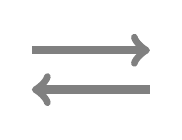
\begin{tikzpicture}[thick]
%\draw [green, ->          ] (0,1) -- (1,1);
%\draw [blue,  -stealth    ] (0,0.8) -- (1,0.8) node [right] {stealth};
\draw [line width=3, -> , color=gray       ] (0,0) -- (1.5,0) node [midway,above]{$\GS$};
\draw [line width=3, -> , color=gray       ] (1.5,-0.5) -- (0,-0.5) node [midway,below]{$\GS$};
%\draw [cyan,  -to         ] (0,0.4) -- (1,0.4) node [right] {to};
\end{tikzpicture}
%\begin{tikzpicture}
%[every node/.style={inner sep=0pt}]
%\node (1) [circle, minimum size=17.5pt, fill=orange, line width=1.25pt, draw=black] at (37.5pt, -25.0pt) {\textcolor{black}{1}};
%\node (2) [circle, minimum size=17.5pt, fill=orange, line width=1.25pt, draw=black] at (37.5pt, -75.0pt) {\textcolor{black}{2}};
%\node (3) [circle, minimum size=17.5pt, fill=lime, line width=1.25pt, draw=black] at (87.5pt, -25.0pt) {\textcolor{black}{3}};
%\node (4) [circle, minimum size=17.5pt, fill=lime, line width=1.25pt, draw=black] at (87.5pt, -75.0pt) {\textcolor{black}{4}};
%\draw [line width=1.25, ->, color=black] (1) to  [in=118, out=242] (2);
%\draw [line width=1.25, ->, color=black] (2) to  [in=302, out=58] (1);
%\draw [line width=1.25, ->, color=black] (2) to  (4);
%\draw [line width=1.25, ->, color=black] (4) to  (3);
%\draw [line width=1.25, ->, color=black] (3) to  (1);
%\end{tikzpicture}
\end{document}
